% Титульный лист (отдельно)
% Лист задания (отдельно)
% Аннотация (отдельно)

% Оглавление
\tableofcontents
\newpage

\section{Введение}
	\textbf{Актуальность темы}. Уже сейчас только объём видео-контента высокого качества (в 4K разрешении) достигает
	колоссальных размеров, а его передача большой аудитории зрителей в режиме реального времени требует поддержания
	масштабной инфраструктуры, затраты на которую будут только рости с повышением качества контента и увеличением числа
	пользователей. Если не начать решать задачу оптимизации систем для вещания видео-трансляций сейчас, то в
	скором будущем такие системы не смогут одновременно обеспечивать качественный сервис для своих зрителей и в тоже
	время оставаться рентабельными. Для решения поставленной задачи можно использовать несколько подходов. Одним из них
	является переход от традиционной клиент-серверной модели к модели одноранговых сетей. Именно этот подход лежит в
	основе системы, описываемой в работе.

	\textbf{Цель работы} заключается в разработке P2P-системы для организации вещания видео-трансляций в режиме
	реального времени с использованием мобильного приложения. В данной работе демонстрируется один из вариантов
	построения системы на базе одноранговых сетей для передачи потокового контента между пользователями, которая
	позволит большому числу участников вести  видео-трансляции в режиме реального времени, а основными узлами
	инфраструктуры системы выступают сами устройства зрителей. Главные особенности такого подхода заключаются в:
	\begin{itemize}
		\item значительном снижаении числа централизованных узлов, что непосредственно влияет на отказоустойивость
		системы в целом, а так же на стоимость поддержки системы;
		\item организации системы, управление которой принадлежит самим пользователям, а не ограниченному кругу лиц.
	\end{itemize}

	\textbf{Объектом исследования} являются P2P-системы для организации обмена видеоконтентом между узлами в режиме
	реального времени.

	\textbf{Предметом исследования} являются методы организации передачи видеоконтента в режиме реального времени в
	P2P-системах.

	\textbf{Научная новизна}. На момент разработки системы существует ряд исследований по данному направлению, но
	большинство из них носит академический характер в виде исследовательских работ и не были апробированы в реальных
	условиях, а только были реализованы прототипы для проведения тестирования ({\color{red} ...}). Лишь небольшое число
	систем, описанных в исследовательских работах, было воплощено в готовые продукты для конечных пользователй, но и они
	не пока не стали широко распространены (например, {\color{red} ...}). По этому, учитывая сложившуюся ситуацию, я
	считаю, что разработка системы, которая носит практическую ценность, а не только исследовательскую, является важным
	шагом на пути распространения систем такого типа, так как по настоящему корректность описанных моделей можно лишь
	проверить на практике, и есть вероятность, что часть моделей может оказаться непригодной к реальным условиям.

% Основная часть
\section{Анализ предметной области}

	В последнее время стремительно растёт популярность приложений, в которых используется потоковое видео-вещание.
	В качестве примеров можно привести сервисы YouTube и Netflix. Только у Netflix насчитывается более 100 миллионов
	пользователей, которые просматривают более 125 миллионов часов фильмов и сериалов каждый день. Но так стремительно
	растёт не только пользовательская база. Трафик, генерируемый просмотром потокового видео-контрента высокого
	разрешения, достигает до 50\% всего трафика на территории Соединённых Штатов Америки, из которых 20\% принадлежат
	трафику Netflix. Для предоставления сервиса потокового вещания в таких масштабах Netflix использует ресурсы
	сторонних CDN, а с 2011 года разворачивает свою выделенную инфраструктуру CDN в рамках проекта Open Connect для
	снижения эксплуатационных расходов.

	Помимо CDN существует и другой способ доставки контента до пользователей: одноранговые (пиринговые) сети.
	Главная особенность таких сетей заключается в том, что участник сети одновременно является и получателем контента,
	и сам принимает участие в передаче контента другим заинтересованным участникам. Таким образом, ресурсы каждого из
	участника становятся частью общедоступных ресурсов всего сервиса. Это позволяет быстро и дёшево масштабировать
	сервис в зависимости от числа пользователей, что является важным показателем для сервисов потокового видео-вещания.
	Резкое изменение числа пользователей сервиса обуславливается привычками пользователей. Например, в вечерние часы
	число пользователей резко возрастает. Так же резкий рост нагрузки на систему может возникать в ходе проведения
	различных мероприятий (спортивные игры, концерты, празники).

	На протяжении последних лет в научном сообществе было предложено множество различных схем организации пиринговых
	сервисов обмена видео-контентом по запросу, так и в режиме реального времени. Но до сих пор остаётся открытым вопрос
	об архитектуре, которая наилучшим образом подойдёт для решения большинства задач. Некоторые авторы утверждают, что
	mesh-архитектура обладают наилучшей производительностью, тогда как tree-архитектура лучше подходит для организации
	вещания в режиме реального времени. Главный вопрос заключается в выборе архитектуры, в системе на базе которой будут
	наименьшие издержки на накладные расходы, наименьшее время на задержку перед вещанием и наименьшее число прерываний
	во время вещания. Некоторые авторы предлагают гибридные системы разных видов, когда в системе или берутся лучшие
	идеи из разных архитектур и совмещаются вместе (что повышает сложность таких систем и издержки на накладные расходы),
	или в зависимости от текущих условий работы система выбирает наиболее подходящую архитектуру организации системы.
	На рисунке \ref{img:p2p-mechanisms} представленно отображение проблемы, когда каждый из типов архитектур лучше
	подходит под те или иные условия и нет единого универсального решения.

	\begin{figure}[h]
		\center{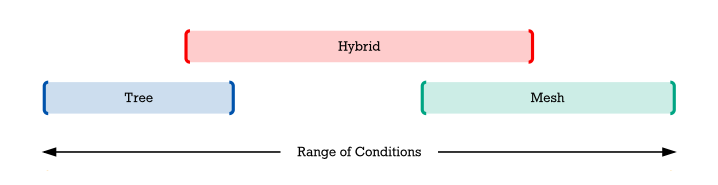
\includegraphics[width=0.8\linewidth]{p2p-mechanisms.png}}
		\caption{Механизмы организации системы в зависимости от условий}
		\label{img:p2p-mechanisms}
	\end{figure}

	\subsection{Цель работы и исследовательские задачи}
	Целью данной работы является разработка системы для проведения видео-трансляций в режиме реального времени между
	пользователями. Ключевой особенностью этой системы является применение принципов построения одноранговых сетей к
	организации взаимодействия участников между собой. В качестве основного программного обеспечения системы выступает
	приложение для платформы iOS, которое позволяет участникам быть как ведущим трансляций, так и зрителем.

	Для достижения поставленной цели были рассмотренны следующие задачи:
	\begin{itemize}
		\item анализ литературы в области существующих решений P2P-систем для ведения трансляций (такой анализ позволил
		определить ключевые аспекты архитектуры рассматриваемых систем и определить потенциальные возможности и
		недостатки этих систем);
		\item проектирование системы в целом и архитектруы мобильного приложения в частности (при решении этой задачи
		было получено описание всех необходимых модулей системы, схема их взаимодействия, а так же модель для данных,
		которые используются при передаче информации от одного модуля к другому);
		\item разработка модуля системы, отвечающего за формирование и поддержание связей между участниками и передачу
		данных между ними;
		\item разработка мобильного приложения для пользователей, с помощью которого они могут вести свои
		видео-трансляции или могут быть зрителями других трансляций;
		\item тестирование разработанного ПО для получения данных об эффективности применяемых подходов в его создании.
	\end{itemize}

	\subsection{Традиционные способы организации видео-трансляций}
	Первым, что приходит на ум при упоминании традиционных систем передачи контента с большой аудиторией - это
	телевизионное вещание. В его основе лежит простая идея - транслировать контент всем, кто находится в пределах
	досягаемости (\textit{broadcast}). Но такой подход не применим для передачи контента через Интернет, так как лишь
	заинтересованные лица должны получать контент (\textit{multicast}). При таком подходе система может быть
	организована с использованием паттерна издатель/подписчик, когда заинтересованные участники объеденяются в группы и
	получают новый контент предназначенный конкретной группе. В контексте систем видео-трансляций в режиме реального
	времени этот подход является ключевым и может быть реализован на различных уровнях сетевой модели OSI.

	Существует два подхода к организации multicast в рамках стека TCP/IP: Internet Protocol Multicast и Application
	Level Multicast (ALM). На рисунке \ref{img:ip-multicast-vs-application-multicast} представленно схематическое изображение
	каждого из подходов, а далее по тексту приведенно более подробное описание каждого подхода.

	\begin{figure}[h]
		\center{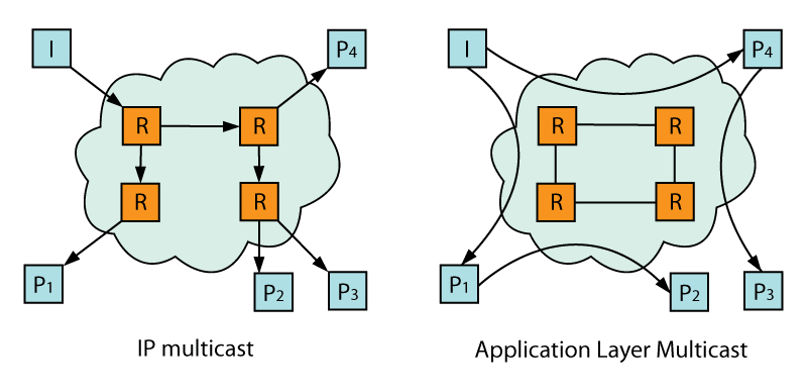
\includegraphics[width=0.8\linewidth]{ip-multicast-vs-application-multicast.png}}
		\caption{Схема взаимодействия узлов при работе через IP Multicast и ALM}
		\label{img:ip-multicast-vs-application-multicast}
	\end{figure}

		\subsubsection{Internet Protocol Multicast}
		Протокол сетевого уровня модели OSI IP уже включает в себя поддержку многоадрессного вещания
		(\textit{multicast}). Но несмотря на высокую производительность этой технологии по сравнению с другими, она не
		стала массово распространенной из-за дополнительных требований к роутерам в сети Интернет и ограниченности
		доступных адресов для организации групп пользователей. В рамках одной автономной системы эта технологий может
		использоваться для организации IP-телевидения (IPTV), но не в рамках глобального Интернета для организации
		видео-трансляций.

		В первую очередь, в IP multicast в рамках одной группы может быть несколько источников, что подходит
		для организации видео-конференций, но не обязательно для видео-трансляций. Передача данных устроена таким
		образом, что дублирование пакетов данных происходит только если это действительно требуется, что положительно
		влияет на пропускную способность системы. Каждый роутер в системе должен решать задачу поддержания сведений об
		участниках групп и координировать передачу данных между ними, что отличается от других задач роутера, для
		которых не требуется поддержания состояний. Для добавления новых возможностей, таких как биллинг или управление
		пользователями, необходимо загрузить эти данные во все устройства, принимающие участие в обмене информацией в
		системе. Это возможно лишь в рамках одного интрент-провайдера.

		\subsubsection{Application Level Multicast}
		Для преодоления проблем развёртывания систем с использованием IP multicast, в настоящее время \textit{multicast}
		реализуют на уровне приложения (Application Level Multicast). В приложении описывается протокол, с
		использованием которого организуется передача данных. Тогда как в IP multicast пересылкой и дублированием
		пакетов занимаются роутеры, в ALM этим занимаются конечные устройства пользователей. Коммуницирование между
		конечными устройствами происходит с использованием только IP unicasts, в связи с чем на промежуточные устройства,
		такие как роутеры, не накладываются дополнительные ограничения. Но если сравнивать использование IP unicasts с
		IP multicast, то в ALM появляется дополнительный накладной трафик, так как пакеты с одним контентом могут
		пересылаться по одним и тем же направлениям несколько раз.

		С точки зрения P2P-систем, ALM подходит под это определение, так как узлы предоставляют ресурсы, такие как
		пропускная способность и вычислительная мощность, друг другу. Архитектура \textit{multicast}-системы может быть
		централизованной или полностью распределённой, в зависимости от сценария использования приложения. Одним из
		примеров систем общего назначения ALM, построенным на основе Distributed Hash Table (DHT), является Scribe, в
		которой отсутствуют централизованные элементы.

		Также нужно отметить разницу между используемыми топологиями в IP multicast и ALM. IP multicast всегда
		использует \textit{spanning tree} для организации вещания несколькими участниками в рамках одной группы, а в ALM
		может использоваться любая сетевая топология. Так, для предотвращения дублирования и избежания не нужных
		пересылок, большинство систем поддерживают список в виде дерева для распространения пакетов данных. Для ведения
		трансляций в режиме реального времени требуется высокая пропускная способность и низкие задержки при передачи
		данных от источника к участникам, что влияет на выбор подходящей топологии при построении системы.

	\subsection{Пиринговое вещание}
	P2P-системы для видео-трансляций в режиме реального времени являются подмножеством ALM-систем, в которых
	распространение контента от источника реализовано на уровне приложения. Но в отличии от стандартных ALM-систем,
	P2P-системы включают конечных пользователей в общую схему доставки контента. Таким образом, каждый пользователь
	вносит вклад в распространение контента, который он получает от других пользователей, предоставляя свои ресурсы.
	Это требует координации между пользователями, что бы быть увереным, что каждый из участников получит пакеты данных,
	требуемые для декодирования видео-потока. Существующие P2P-системы можно разделить на \textit{tree-based},
	\textit{mesh-based} или \textit{hybrid}, в зависимости от их топологии сети.

		\subsubsection{Tree-based topologies}
		Tree-based системы по строению схожи с дизайном IP multicast систем, в которых узлы образуют дерево, исходящее
		от источника. Такое строение обеспечивает низкие задержки и корректный порядок пакетов при передачи данных.
		Новые пользователи, при подключении, занимают своё место в дереве в соответствии с протоколом построения
		оверлейной сети. Источник посылает пакеты своим дочерним узлам, тем в свою очередь пересылают своим дочерним
		узлам и так далее. Так как данные пересылаются от источника к листьям по дереву в порядке их отправления, то не
		требуется механизм планирования доставки пакетов. Вместо этого какждый узел просто пересылает все полученные
		пакеты своим дочерним узлам. Такой подход к организации передачи данных называют \textit{push-based}. Так как
		узлы в системе расположены в виде дерева, то возникает вопрос в выборе оптимального соотношения между шириной и
		высотой дерева. Чем дерево шире, тем меньше его высота, и данные быстрее доходят до листьев дерева. Но в то же
		время это повышает ветвление в промежуточных узлах, что означает увеличение нагрузки в этих узлах.

		\begin{figure}[h]
			\center{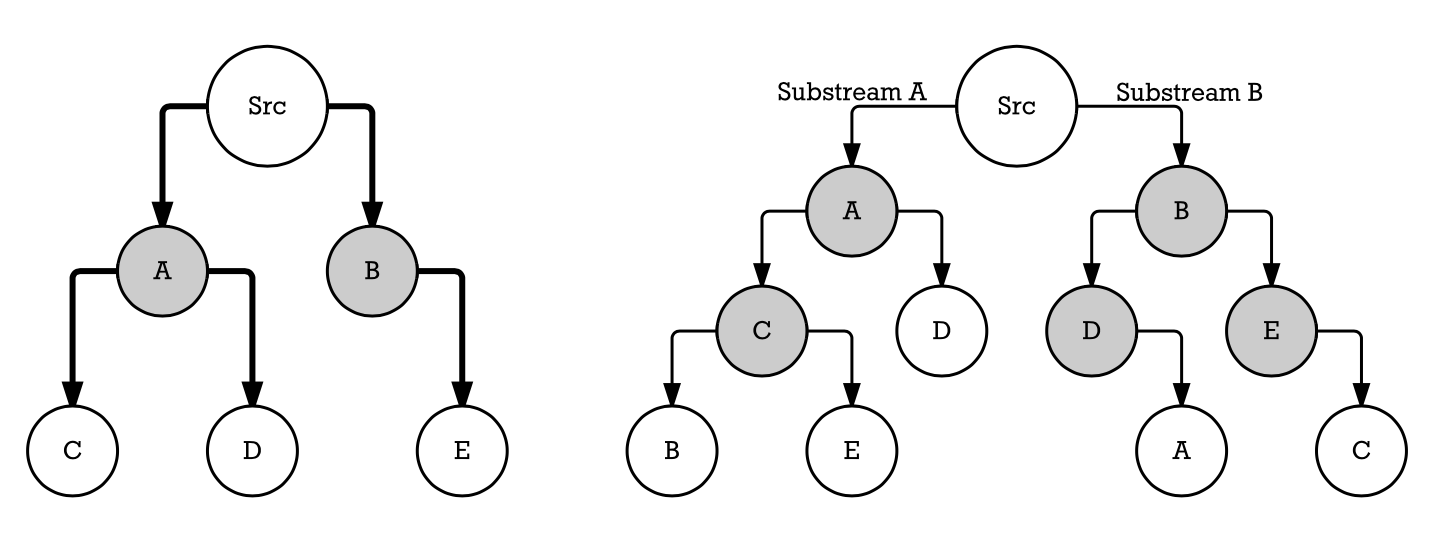
\includegraphics[width=0.8\linewidth]{tree-based-system.png}}
			\caption{Организация оверлейной сети в tree-based системах}
			\label{img:tree-based-system}
		\end{figure}

		При рассмотрении ситуации, близкой к идеальной, в которой узлы надёжны и не покидают сеть во время трансляции,
		в системе почти отсутствуют накладные расходы на поддержание оверлейной сети. В этом случае пути распространения
		пакетов стабильны и не изменяются. В действительности, таких условий почти не бывает, так как узлы являются
		нестабильными и набор узлов в сети часто изменяется, что значительно влияет на производительность tree-based
		систем. Для поддержания актуального состояния древовидной структуры узлов необходимо регулярно восстанавливать
		связанность дерева в случае выбывания узлов, что может привести к значительным накладным расходам. В случае,
		если дерево покидает промежуточный узел, то все его потомки не смогут получать данные от источника. Для
		гарантирования непрерывного воспроизведения трансляции, узлы должны определять возникновение таких ситуаций и
		переподключаться к рабочим узлам дерева. Так же требуется, что бы узлы кешировали часть пакетов для последующей
		их передачи узлам, чьи родительские узлы выбыли из дерева. Если обнаружение и восстановление повреждённых связей
		в дереве не будет надёжным и быстрым, то узлы вниз по дереву будут испытывать задержки при воспроизведении в
		следствии отключения от потока данных. Как только начинает активно изменяться дерево узлов, сразу увеличивается
		сложность быстрого и надёжного восстановления связей в дереве.

		Для повышения надёжности системы во время активного изменения дерева узлов, а некоторых системах используется
		несколько деревьев. Разница между системами с одним деревом и несколькими показана на рисунке
		\ref{img:tree-based-system}. Обе оверлейные сети состоят из источника (S) и пятерых зрителей (A-E). В системе с
		одним деревом используются ресурсы только узлов A и B. В системе с несколькими деревьями поток данных от
		источника разделён на два, и для каждого из них используется своё дерево. Каждый из узлов включён в каждое из
		деревьев только один раз, что позволяет каждому из пользователей предоставлять свои ресурсы системе. Совместо с
		применением MDC для декодирования видео становится возможным передача независимых частей трансляции по каждому
		из дереьев, которые могут быть декодированы независимо друг от друга. Таким образом решения на базе нескольких
		деревьев эффективнее используют ресурсы узлов и имеют повышенную стабильность в сравнении с системами с одним
		деревом.

		Для большинства систем, в которых используются деревья, необходим централизованный сервис для поддержания дерева
		и восстановления после сбоев. Часто в качестве такого узла выступает источник трансляции. В случае, когда дерево
		стабильно, то накладные расходы на выполнения второстепенных задач значительно меньше расходов ресурсов на
		ведение трансляции. Но когда дерево нестабильно, этот узел может стать узким местом в системе. Когда изменение
		потоков данных в дереве происходит слишком часто, и дочерним узлам необходимо дополнительно запрашивать
		недостающие пакеты, подход push-based становится неэффективным. В таких условиях подход \textit{mesh-based}
		может оказаться эффективнее для построения более надёжной системы.

		\subsubsection{Mesh-based topologies}
		В mesh-based системах участники соединены между собой краткосрочными соединениями. Они обмениваются друг с
		другом информациий о доступном контенте на каждом из узлов и запрашивают друг у друга недостающие части на
		основе этих данных. Механизм, когда сам получатель запрашивает недостающие части, называется \textit{pull-based}.
		Для получения сведений о новых узлах в системе, участники регулярно обмениваются информацией о их текущих
		соседних узлах. В случае, когда узел узнаёт о новых участника в системе, он может инициировать новое соединение.
		На рисунке \ref{img:mesh-based-system} показана оверлейная топология mesh-based систем в два разных момента
		времени. Пунктирными линиями обозначены соединения, а оттенок узлов отражает число соединений с соседними узлами.
		В приведённом примере соединения двунаправленны, то означает обмен данными в обе стороны с использованием одного
		соединения. В большинстве mesh-based систем для видео-трансляций в режиме реального времени узлы не инициируют
		исходящих соединений, а только поддерживают входящие.

		\begin{figure}[h]
			\center{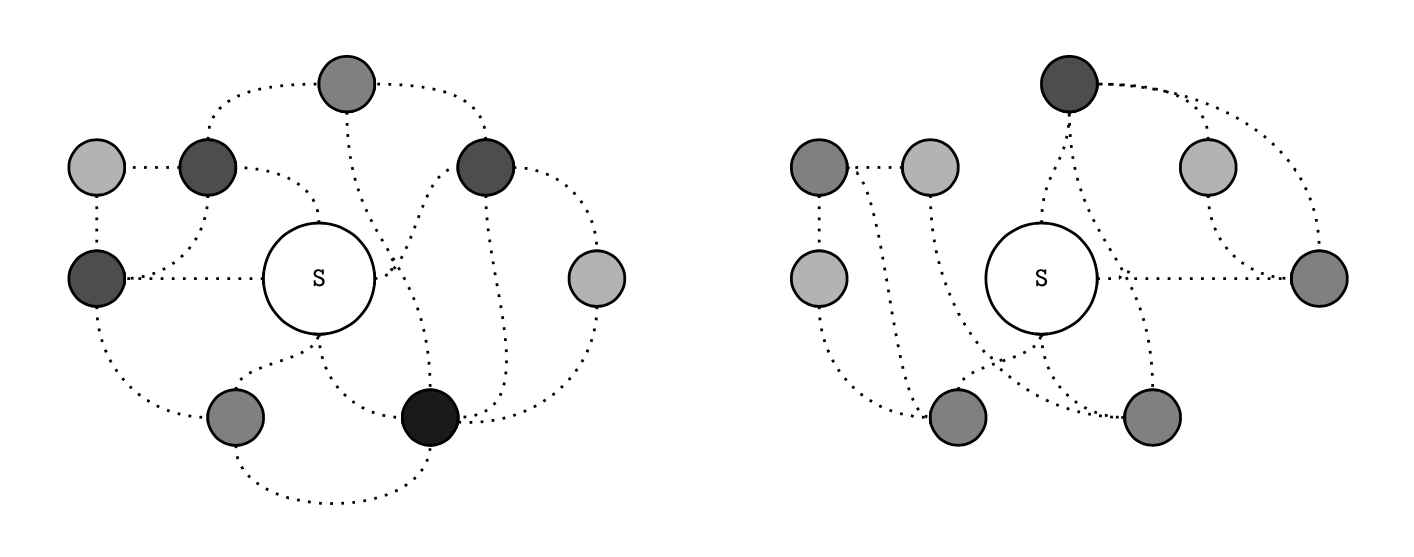
\includegraphics[width=0.8\linewidth]{mesh-based-system.png}}
			\caption{Организация оверлейной сети в mesh-based системах}
			\label{img:mesh-based-system}
		\end{figure}

		Узлы в mesh-сетях как правило поддерживают соединение до тех пор, пока оно используется для передачи данных
		трансляции. Если отправитель не содержит боьше нужных получателю пакетов данных, то соединение может быть
		закрыто и установлено новое с другим узлом. Время существования соединения не влияет на схему планирования
		передачи данных в pull-based системах, так как регулярно каждый узел сообщает сведения о доступных у него
		пакетах данных соседним участникам. И в случае, если не удалось загрузить данные с одного узла, то они
		будут запрошены с другого узла, который ранее сообщих о их доступности. Из-за такого поведения mesh-based
		системы более устойчивы к регулярной смене узлов в оверлейной сети, но в то же время появляются дополнительные
		накладные расходы и увеличиваются задержки на передачу данных.

		\begin{figure}[h]
			\center{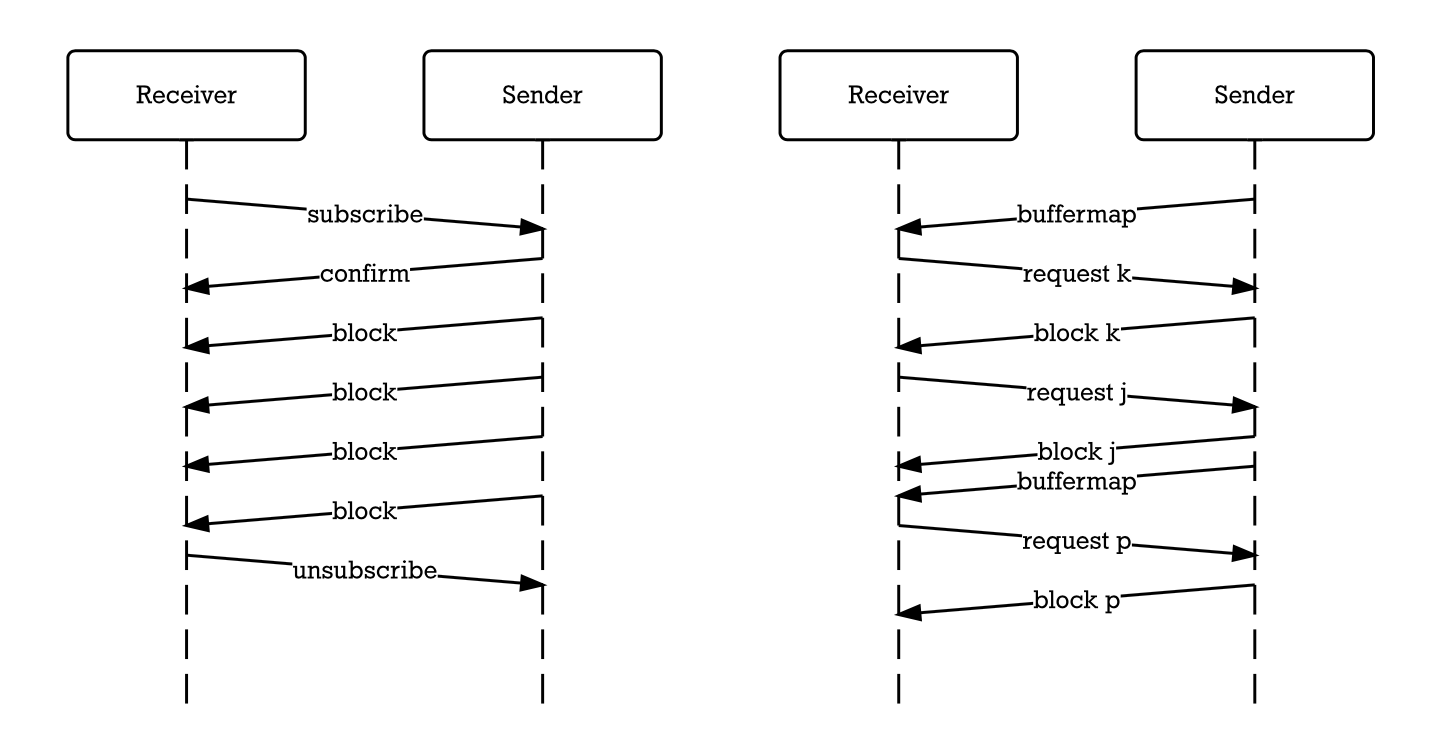
\includegraphics[width=0.8\linewidth]{scheduling-scheme.png}}
			\caption{Схемы планирования распространения контента в push-based системах (слева) и в pull-based системах
					(справа)}
			\label{img:scheduling-scheme}
		\end{figure}

		Обе схемы планирования распространения контента показаны на рисунке \ref{img:scheduling-scheme}. Так, в
		push-based системах получатель отправляет запрос источнику на установку соедиения, и после получения
		подтверждения, он будет получать новые пакеты данных от источника, как только они станут доступны отправителю.
		Когда получатель решит, что он больше не хочет получать данные от источника, то он просто закроет соединение.
		В pull-based системах в место установления соединения источник отправляет информацию о доступных пакетах данных
		(buffermap) получателю, а тот на основе полученной информации запрашивает необходимые ему пакеты данных. Для
		каждого пакета данных получатель отправляет отдельный запрос. По прошествию небольшого отрезка времени,
		источник отправляет обновлённую информацию о доступных пакетах, которые он получил за время после отправки
		предыдущей информации.

	\subsection{Обзор аналогов}
		\subsubsection{P2P tree-based system}

		\textit{Overcast}

		Одним из примеров систем с единым деревом в основе оверлейной сети является Overcast. В этой системе
		создаётся и поддерживается единое дерево, которое имеет высокую пропускную способность для передачи контента от
		источника до получателей. Алгоритм, отвечающий за построение дерева, выбирает такое строение, при котором будет
		максимальной пропускная способность от источника до каждого листа. Это достигается путём поддержания небольшого
		числа соединений на промежуточных узлах, что отрицательно влияет на задержки в узлах-листах. Overcast не был
		спроектирован для видео-трансляций в режиме реального времени, а его задачей является передача контента большим
		группам пользователей, где допустимы задержки до 15 секунд. Основной целью является доставка контента не на
		прямую конечным пользователям (участникам оверлейной сети), а вместо этого конечные пользователи получают
		контент с узлов сети Overcast используя протокол Hypertext Transfer Protocol (HTTP). Таким образом эту
		систему можно сравнить с CDN.

		Дизайн рассматриваемой системы предполагает, что узлы в системе являются стабильными, и не часто присоединяются
		или покидают сеть. Это позволяет протоколу более эффективно оптимизировать дерево узлов. Новые узлы в системе
		добавляются в дерево как можно дальше от источника, так как задержка в системе не является критичным фактором,
		но в то же время это позволяет поддерживать небольшое число соединений на промежуточных узлах, благодаря чему
		достигается высокая пропускная способность. Со временем характеристики каждого из соединений могут изменяться,
		поэтому в системе предусмотрен механизм перестройки дерева для балансировки нагрузки между узлами, который так
		же срабатывает при выходе из строя родительских узлов.

		\textit{CoopNet}

		Система CoopNet является одной из первых, в которой P2P-подход не полностью заменяет централизованный подход
		для решения задач видео-трансляций, а совмещает в себе принципы из двух подходов. Авторы предположили, что
		узлы в системе могут часто как присоединяться, так и отключаться от оверлейной сети, что делает её непостоянной.
		Одиним из решений проблемы устойчивости к потере пакетов было использование видео-кодека MDC и рассылка
		независимых пакетов данных по разным деревьям в сети для возможности независимого декодирования потока на
		узле зрителя. Для поддержания консистентного состояния дерева используется централизованный узел в виде
		источника, который выполняет всю необходимую работу поддержания топологии. Централизованный подход к построению
		оверлейной сети позволяет CoopNet оптимизировать дерево узлов в соответствии с текущими условиями.
		В представленном отчёте о работе системы видно, что применение системы позволило значительно снизить нагрузку
		на центральный сервер при массовом прибытии новых пользователей.

		Обычно P2P-системы рассматриваются как полностью децентрализованные, но в случае с системами видео-трансляций в
		режиме реального времени всегда будет центральный узел - источник, и в случае его выхода из сети в системе не
		будет доступно никакого контента и уже будет не так важно, полностью децентрализованная система или нет.
		Поэтому, выбор авторов использовать централизованный узел для выполнения ряда задач допустим и не накладывает на
		систему дополнительных ограничений.

		\textit{SplitStream}

		Система SplitStream отличается от других решений тем, что не строит свою оверлейную сеть, а вместо этого
		использует DHT и системы группового общения, построенные поверх DHT. Авторы используют в своей работе SCRIBE и
		PASTRY, но так же могут быть использованы и другие системы. Изначально система SCRIBE не проектировалась для
		передачи больших объёмов данных, но использование нескольких деревьев для передачи пакетов данных решает данную
		проблему.

		Применение multicast-групп из SCRIBE в SplitStream накладывает ограничение, что все узлы в системе получают
		данные только одной трансляции. По утверждениям авторов, такой подход позволяет балансировать нагрузку между
		узлами и лучше справляться с наплывом новых узлов в сети. Производительность SplitStream напрямую зависит от
		используемых решений DHT и системы группового общения, не имея своего дополнительного механизма по
		восстановлению оверлейной сети в случае возникновения сбоев.

		\textit{Stanford Peer-to-Peer Multicast}

		Протокол Stanford Peer-to-Peer Multicast (SPPM) использует ключевые идеи двух уже рассмотренных выше систем:
		CoopNet и SplitStream. В нём также поддерживаются несколько деревьев, но не используется MDC кодирование.
		Вместо этого, если при первоначальной передаче от источника к получателю пакет не был доставлен, то получатель
		запрашивает недостающий пакет сам у родительского узла. Если родительский узел в течении определённого времени
		не переслал нужный пакет, то требуемый пакет запрашивается у других узлов. SPPM оптимизирован для передачи
		видео в формате H.264/AVC, выставляя более высокий приоритет некоторым пакетам (ключевые кадры видео) в
		зависимости от их содержимого.

		\subsubsection{P2P mesh-based system}

		\textit{CoolStreaming/DONet}

		DONet относится к классу систем, в которых узлы обмениваются информацией о доступном контенте и уже на её основе
		происходит построение связей между узлами. Во время трансляции видео-поток делится на пакеты, и узлы сообщают
		соседним узлам о доступных у них пакетах с помощью \textit{buffer maps}. Для воспроизведения видео-потока в
		режиме реального времени необходимы только пакеты для текущего воспроизведения, поэтому в buffer maps передаётся
		информация только о тех пакетах, в которых есть данные для текущего момента воспроизведения, или более новые,
		для последующего воспроизведения. Размер буфера напрямую влияет на задержку воспроизведения контента на узле по
		сравнению с источником. В DONet допускаются задержки до одной минуты, что означает большой размер буфера.
		Buffer maps представляет битовый список, где каждый бит означает наличие того или иного пакета, и идентификатор
		первого пакета, предназначенного для синхронизации с другими узлами. Обмен пакетами и buffer maps может
		происходить в обе стороны, поэтому в такой оверлейной сети нету родительских отношений, в все узлы являются
		соседями друг друга.

		По утверждению авторов, эффективность передачи контента зависит от алгоритма планировщика. Для непрерывного
		воспроизведения трансляции необходимо иметь возможность выставлять более высокий приоритет пакетам, которые
		необходимы для текущего воспроизведения. Так же необходимо учитывать текущую нарузку на узлы, что бы не
		возникало ситуаций, когда они перегруженны. Для выполнения обоих условий в DONet сначала запрашиваются пакеты,
		доступные только одному соседнему узлу, а затем для получения остальных пакетов отправляются запросы наименее
		загруженным узлам.

		DONet использует в качестве системы управления узлами систему SCAMP. Используя SCAMP, узлы регулярно рассылают
		сообщения о своих соседних узлах по оверлейной сети. Эта информация сохраняется в кеше узлов и позволяет
		перестраивать сеть для повышения общей пропускной способности в системе.

		\textit{Prime}

		В системе Prime узлы устанавливают соединения между собой случайным образом, образуя mesh-сеть. Отношение
		входящих и исходящих соединений на каждом из узлов определяется динамически, в зависимости от пропускной
		способности каждого узла. Вся передача данных в системе разделена на два этапа: \textit{diffusion} и
		\textit{swarming}.

		В момент генерации новых сегментов трансляции на источнике они ещё не доступны другим узлам в сети. На этапе
		diffusion вновь сгенерированные сегменты распространяются таким образом, чтобы каждый из узлов получил хотя бы
		часть пакетов сегмента. В Prime узлы активно распространяют информацию о доступных их пакетах, которые будут
		отправлены соседним узлам в ответ на их запрос. Все узлы в оверлейной сети разделены на уровни, который зависит
		от степени удалённости узла от источника.

		На этапе swarming происходит получение недостающих пакетов данных путём их запроса у соседних узлов. Для этого
		могут быть использованы как уже ранее установелнные соединения между узлами, так и сформированны новые, которые
		позволят сбалансировать нагрузку между узлами.

		Общую схему оверлейной сети в системе Prime можно увидеть на рисунке \ref{img:prime-overlay}.

		\begin{figure}[h]
			\center{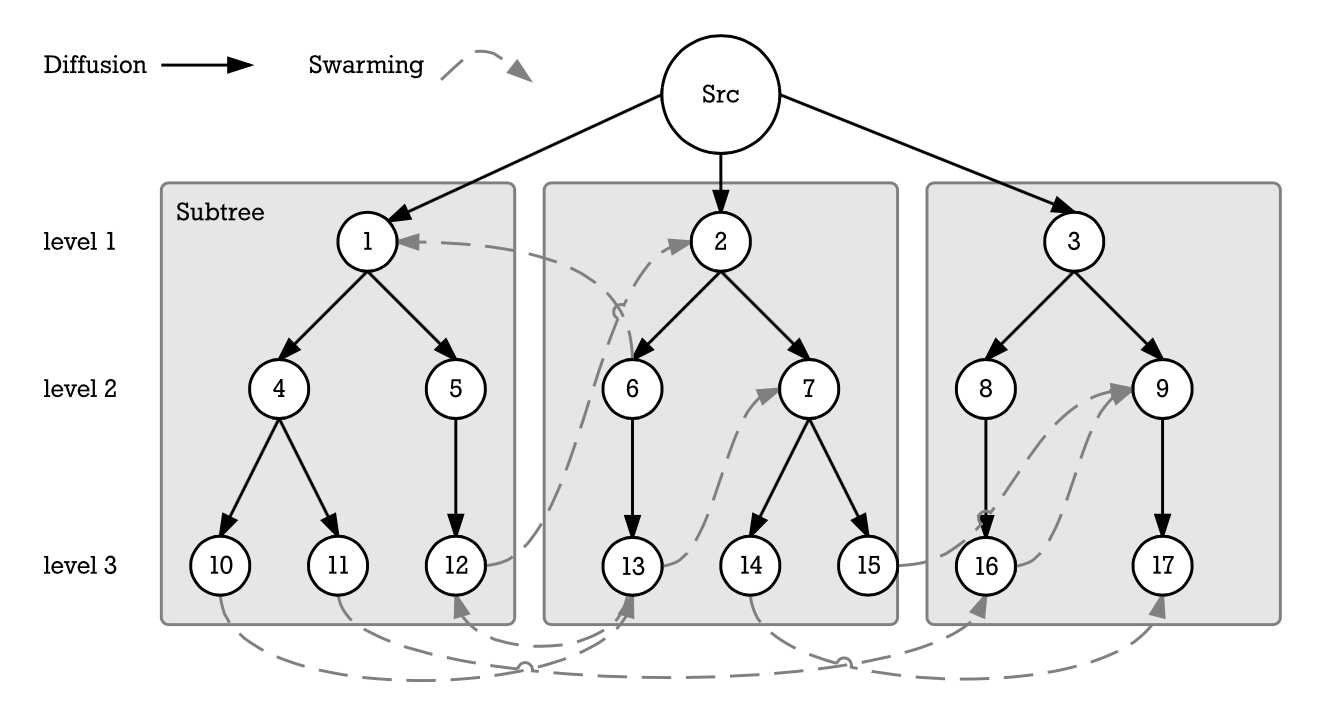
\includegraphics[width=0.8\linewidth]{prime-overlay.png}}
			\caption{Схема оверлейной сети в системе Prime}
			\label{img:prime-overlay}
		\end{figure}

		\subsubsection{Hybrid system}

		\textit{mTreebone}

		В системе mTreebone в построении дерева принимают участие только стабильные узлы, которые уже присутствуют в
		сети определённое время, а все новые узлы считаются нестабильными и могут быть только листьями дерева. Для
		повышения эффективности передачи данных в системе по сравнению с системами с одним деревом, в дополнении к
		основному дереву в mTreebone строится оверлейная mesh-сеть между узлами, которая помагает в построении дерева и
		его восстановлении и в передаче пакетов данных. Так как при построении дерева учитываются только стабильные узлы,
		то накладные расходы на поддержание сбалансированного дерева находятся в допустимых границах.

		На рисунке \ref{img:mtreebone-overlay} показан пример построения оверлейной сети в mTreebone.
		\begin{figure}[h]
			\center{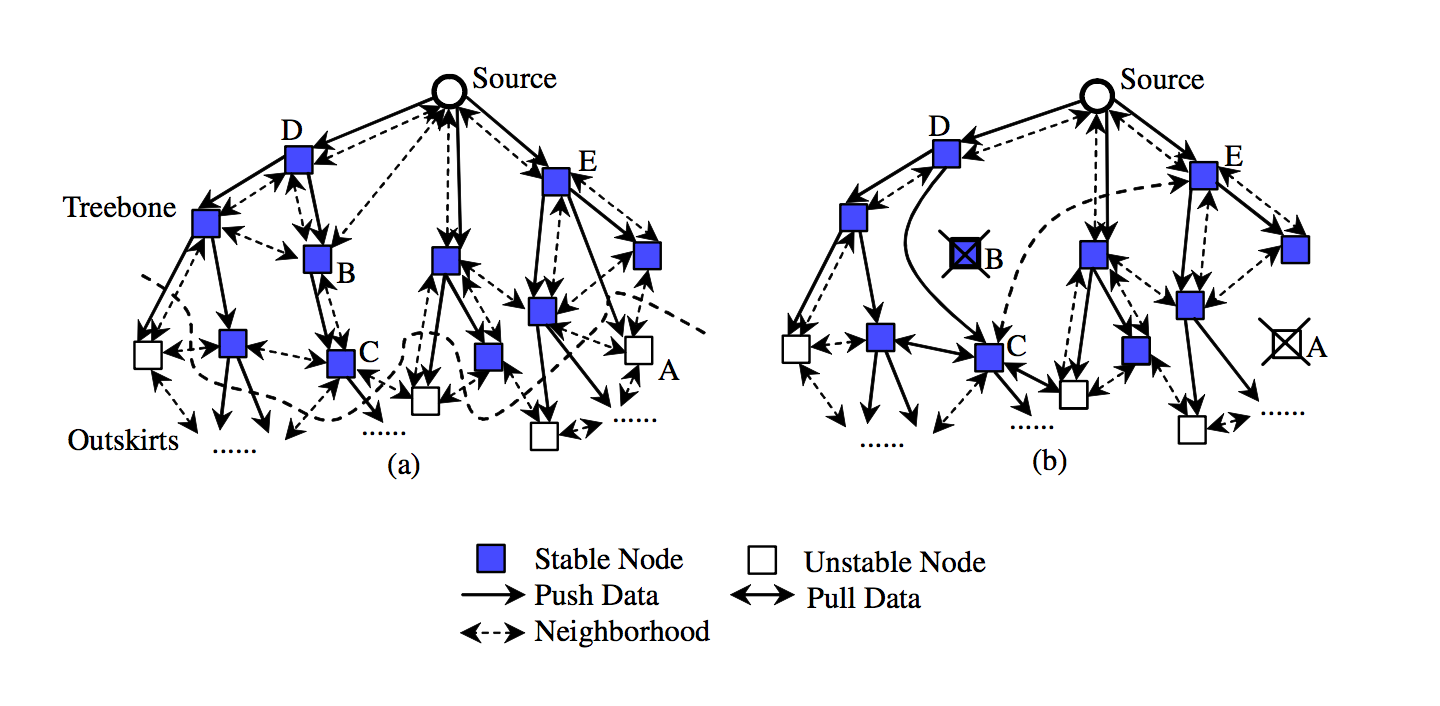
\includegraphics[width=0.8\linewidth]{mtreebone-overlay.png}}
			\caption{Схема оверлейной сети в системе mTreebone. (a) Оверленая сеть, (b) Перестроение сети после
			выхода из неё узлов}
			\label{img:mtreebone-overlay}
		\end{figure}

		Определение стабильных узлов происходит на основе промежутка времени, в течении которого они принимают участие в
		работе системы. Узел становится стабильным после того, как время его работы в сети превысит заданный параметр.
		Этот параметр конфигурируется не статически, а зависит от общего времени ведения трансляции.

		Для снижения задержек при передачи данных между узлами необходимо поддерживать дерево в сбалансированном виде и
		как можно короче. Для этого в mTreebone используется два алгоритма:
		\begin{itemize}
			\item если у узла больше потомков, чем у его родительского узла, то этот узел передвигается выше по дереву и
			его родительский узел становится его потомком;
			\item узел будет всегда стараться минимизировать расстояние между ним и источником, если позволяет
			пропускная способность родительского узла.
		\end{itemize}

		Основным способом передачи данных в системе является push-based подход, но в случае, когда на узле отсутствует
		нужный пакет данных, то он может послать запрос по mesh-сети. Для избежания пересылки дублирующих пакетов, узел
		может запросить недостающий пакет лишь после того, как будет получен более новый пакет через дерево.

		\textit{BitTorrent Live}

		BitTorrent Live является одной из немногих систем, реализации которых в виде конечных продуктов доступны
		пользователям. Первая реализация системы была представленна в 2013 году. В основе системы лежит несколько разных
		механизмов, которые используются одновременно. На рисунке \ref{img:btlive-overlay} показан пример оверлейной
		сети. Весь процесс передачи данных трансляции можно разделить на три этапа: передача частей видео-потока от
		источника до клубов (\textit{clubs}), передача данных между участниками клуба и обмен данными с участниками
		других клубов.

		\begin{figure}[h]
			\center{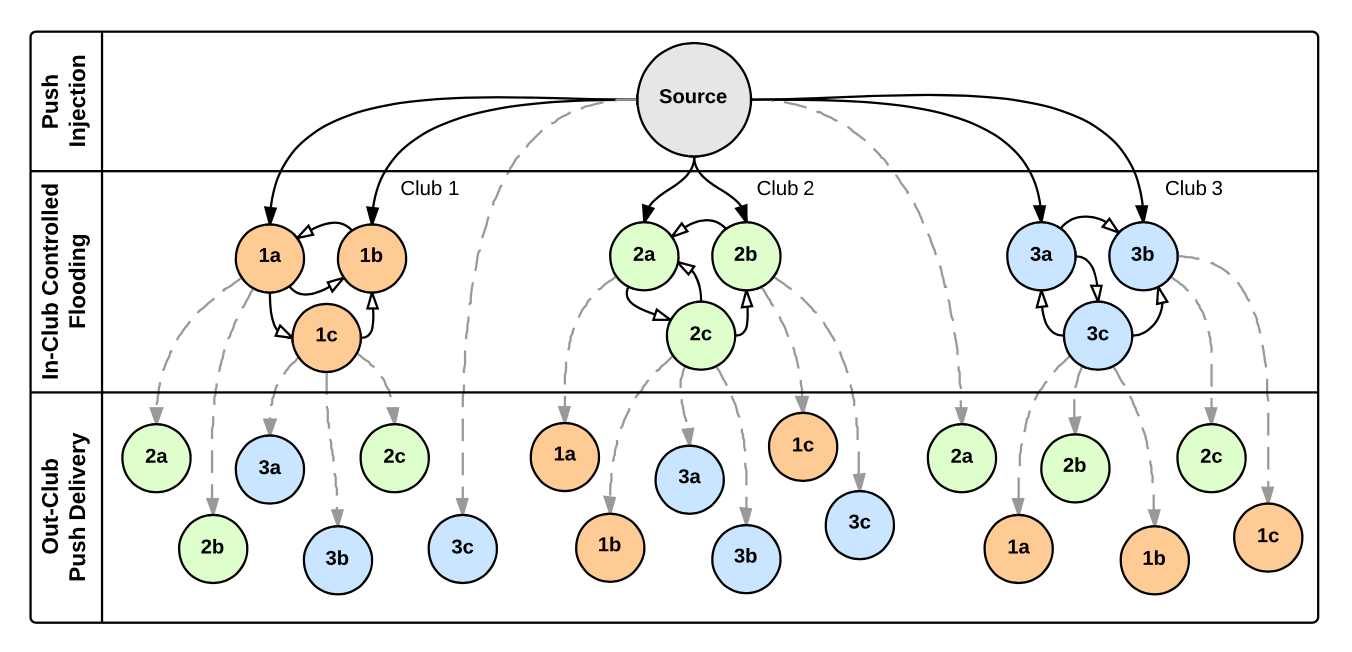
\includegraphics[width=0.8\linewidth]{btlive-overlay.png}}
			\caption{Схема оверлейной сети в системе BitTorrent Live}
			\label{img:btlive-overlay}
		\end{figure}

		В целом, архитектура системы BitTorrent Live позволяет добиться снижения задержек при передачи данных ценой
		пересылки дублирующих пакетов данных. Все узлы в сети разделены на равные группы (клубы). При отправке
		видео-потока источник разделяет его на несколько частей, в соответствии с количеством клубов. Каждому клубу
		отправляется только своя часть общих данных. После получения части потока участники клуба активно начинают
		распространять между собой эту часть данных, используя протокол \textit{gossip}. Для снижения вероятности
		получения уже имеющихся у узла данных при получении пакета данных, он уведомляет соседние узлы в клубе, что
		определённый пакет у него уже есть. После того, как большинство узлов в клубе будут иметь свою часть данных,
		пакет данных, предназначенный их клубу, будет рассылаться участникам из других клубов.

		\subsubsection{Результаты сравнения}
		После изучения вышеперечисленных систем была составлена итоговая таблица \ref{tbl:comparison-p2p-model} с
		оценкой каждой системы по четырём ключевым характеристикам.

		\begin{table}[h]
	\small
	\centering
	\caption{-- Результаты сравнения P2P-систем}
	\label{tbl:comparison-p2p-model}
	\begin{tabular}{|l|l|l|l|l|l|l|l|l|}
	\hline
		\multicolumn{1}{|c|}{Система}&
		\multicolumn{1}{ c|}{Топология}&
		\multicolumn{1}{ c|}{Планирование}&
		\multicolumn{1}{ c|}{ПС }&
		\multicolumn{1}{ c|}{НЗ}&
		\multicolumn{1}{ c|}{Н}&
		\multicolumn{1}{ c|}{М}&
		\multicolumn{1}{ c|}{Видео-кодек}\\ \hline
		\multicolumn{1}{|c|}{Overcast (2000)}&
		\multicolumn{1}{ c|}{single-tree}&
		\multicolumn{1}{ c|}{push}&
		\multicolumn{1}{ c|}{$+$}&
		\multicolumn{1}{ c|}{---}&
		\multicolumn{1}{ c|}{---}&
		\multicolumn{1}{ c|}{---}&
		\multicolumn{1}{ c|}{---}\\ \hline
		\multicolumn{1}{|c|}{CoopNet (2002)}&
		\multicolumn{1}{ c|}{multi-tree}&
		\multicolumn{1}{ c|}{push}&
		\multicolumn{1}{ c|}{$\circ$}&
		\multicolumn{1}{ c|}{$+$}&
		\multicolumn{1}{ c|}{$+$}&
		\multicolumn{1}{ c|}{$\circ$}&
		\multicolumn{1}{ c|}{MDC}\\ \hline
		\multicolumn{1}{|c|}{SplitStream (2003)}&
		\multicolumn{1}{ c|}{multi-tree}&
		\multicolumn{1}{ c|}{push}&
		\multicolumn{1}{ c|}{$\circ$}&
		\multicolumn{1}{ c|}{$+$}&
		\multicolumn{1}{ c|}{$+$}&
		\multicolumn{1}{ c|}{$+$}&
		\multicolumn{1}{ c|}{MDC}\\ \hline
		\multicolumn{1}{|c|}{Stanford P2PM (2007)}&
		\multicolumn{1}{ c|}{multi-tree}&
		\multicolumn{1}{ c|}{push/pull}&
		\multicolumn{1}{ c|}{$\circ$}&
		\multicolumn{1}{ c|}{$+$}&
		\multicolumn{1}{ c|}{$+$}&
		\multicolumn{1}{ c|}{$\circ$}&
		\multicolumn{1}{ c|}{AVC or SVC}\\ \hline
		\multicolumn{1}{|c|}{CoolStreaming (2005)}&
		\multicolumn{1}{ c|}{mesh}&
		\multicolumn{1}{ c|}{pull}&
		\multicolumn{1}{ c|}{$\circ$}&
		\multicolumn{1}{ c|}{$\circ$}&
		\multicolumn{1}{ c|}{$+$}&
		\multicolumn{1}{ c|}{$+$}&
		\multicolumn{1}{ c|}{---}\\ \hline
		\multicolumn{1}{|c|}{Prime (2009)}&
		\multicolumn{1}{ c|}{mesh}&
		\multicolumn{1}{ c|}{hybrid}&
		\multicolumn{1}{ c|}{$\circ$}&
		\multicolumn{1}{ c|}{$+$}&
		\multicolumn{1}{ c|}{$+$}&
		\multicolumn{1}{ c|}{$+$}&
		\multicolumn{1}{ c|}{MDC}\\ \hline
		\multicolumn{1}{|c|}{mTreebone (2007)}&
		\multicolumn{1}{ c|}{tree over mesh}&
		\multicolumn{1}{ c|}{push/pull}&
		\multicolumn{1}{ c|}{$+$}&
		\multicolumn{1}{ c|}{$+$}&
		\multicolumn{1}{ c|}{$+$}&
		\multicolumn{1}{ c|}{$+$}&
		\multicolumn{1}{ c|}{---}\\ \hline
		\multicolumn{1}{|c|}{BTLive (2013)}&
		\multicolumn{1}{ c|}{hybrid}&
		\multicolumn{1}{ c|}{push/pull}&
		\multicolumn{1}{ c|}{$+$}&
		\multicolumn{1}{ c|}{$+$}&
		\multicolumn{1}{ c|}{$+$}&
		\multicolumn{1}{ c|}{$\circ$}&
		\multicolumn{1}{ c|}{---}\\ \hline
	\end{tabular}
\end{table}

	\subsection{Определение требований}
	Требования к P2P-системам для организации видео-трансляций в режиме реального времени можно разделить на две
	категории. Пользовательские требования - это те требования, которые относятся к конкретному виду приложения.
	Системные требования являются более обобщёнными и могут применяться к более широкому кругу систем.

		\subsubsection{Пользовательские требования}
		К пользовательским требованиям можно отнести следующие пункты:
		\begin{itemize}
			\item низкая задержка при старте --- пользователь желает начать просмотр как можно быстрее и в случае
			длительной задержки может выйти из системы;
			\item непрерывное воспроизведение трансляции --- если трансляция уже началась, то частые прерывания могут
			спровоцировать закончить просмотр;
			\item наилучшее качество трансляции --- пользователь хочет смотреть трансляцию наилучшего качества, которое
			только доступно;
			\item умеренное потребление ресурсов --- приложение должно потреблять только необходимое колическтво
			ресурсов (процессорное время, пропускная способность канала, заряд аккумулятора).
		\end{itemize}

		\subsubsection{Системные требования}
		К системным требованиям относятся следующие пункты:
		\begin{itemize}
			\item анализ передаваемых данных --- протокол должен понимать формат передаваемых им данных для возможности
			применения необходимых эвристик;
			\item низкие накладные расходы --- небольшой объём вспомогательных данных по отношению к трафику
			видео-трансляции;
			\item высокая пропускная способность системы;
			\item низкая задержка при передаче данных от источника до пользователей;
			\item надёжная доставка данных между узлами;
			\item устойчивость к частым подключениям и отключениям узлов в сети;
			\item масштабируемость.
		\end{itemize}

	\subsection{Выводы по главе}

	В каждой из рассматриваемых работ авторы подтверждают целесообразность использования своих систем на основе
	тестов, проведённых в искуственных условиях. Таким образом сложно оценить, насколько эффективными будут
	их системы в реальных условиях Интернета. Но целью данной работы является разработка системы, которая будет
	работоспособна в сети Интренет и сможет удовлетворить потребности аудитории большого числа пользователей.
	Поэтому вместо использования идей из рассматриваемых работ, были изучены текущие технологии, которые решают
	схожие задачи и уже аппробированы на практике.

	Одной из самых известных P2P-технологий кооперативного обмена данными через Интернет является протокол
	\textit{BitTorrent}. Уже на протяжении 16 лет пользователи активно используют системы на базе этого протокола для
	передачи данных между собой, исключая из цепочки передачи централизованные узлы. По данным на начало 2013 года,
	трафик для передачи данных с использованием протокола BitTorrent составляет 3,35\% от общего мирового трафика
	Интренета. BitTorrent хорошо справляется с задачей обмена файлами, но для эффективной передачи данных
	видео-трансляции в режиме реального времени в том виде, в котором его используют, он не подходит. Поэтому в 2011
	году был представленн стандарт \textit{RFC 7574 Peer-to-Peer Streaming Peer Protocol (PPSPP)}, в котором описывается
	протокол передачи данных, в основе которого лежат идеи из BitTorrent, но доработанный с учётом специфики передачи
	видео-контента. Именно этот стандарт и был взят за основу разработанной системы.

\section{Проектирование P2P-системы для организации видеотрансляций в режиме реального времени}
	\subsection{P2P-протокол для передачи потокового контента}
		% Описание стандарта RFC PPSPP и PPSTP
	% \subsection{Адаптация существующих подходов}
	\subsection{Структура системы}
		\subsubsection{Архитектура системы}
			% Статическое описание системы (виды узлов и их назначение)
		\subsubsection{Архитектура мобильного приложения}
	\subsection{Алгоритм работы системы}
		% Динамическое описание системы (порядок обмена данными между узлами, потоки данных в рамках модуля)
	\subsection{Проектирование пользовательского интерфейса}

\section{Реализация P2P-системы для организации видеотрансляций в режиме реального времени}
	\subsection{Инструменты разработки}
	\subsection{Интеграция}
	\subsection{Подходы к тестированию}
	\subsection{Оценка решений}

\section*{Заключение}
\addcontentsline{toc}{section}{Заключение}
	% Излагается: достоинство работы,a анализ фактически достигнутых результатов, рекомендации относительно возможностей
	% практического применения материалов работы, рекомендации по улучшению (устранению недостатков) и т.д.

% Словарь терминов

% Список литературы
% \bibliographystyle{bibliography/utf8gost705u}
% \bibliography{bibliography/biblio}

% Приложение